The rich information model that we adopt for our platform makes it possible to provide facilities to teachers in order to assist them in  their  pedagogical follow up of students. % This is done at two levels. 
First, it is possible to convey to teachers (part of the) information
that they implicitely have when they do face to face teaching. Second,
additional information can be provided due to the technology
change. Indeed, having all students (guided) tours, answers,  mistakes and,
possibly, teachers annotations stored and accessible in a database
makes it possible to use queries and Data mining techiques to retrieve
pedagogically relevant information for both students and
teachers~\cite{amv03}. Here, we focus on the teacher's point of view. 

We illustrate  our approach   with the Logic-ITA, which can be seen as a particular application case of our platform.

The Logic-ITA is a web-based intelligent teaching assistant system for the domain of
formal proofs in propositional logic currently in use at the Information Technologies School of the University of Sydney.
It provides an
environment where students can practice formal proofs of logic at their
own discretion, receiving step-by-step, contextualised feedback. They
can choose to create new exercises, select exercises in the exercise
database, or ask the system for one adapted to their needs. The system
stores, for each student, every step entered, along with
any mistake the student may have made and collates all this
information into a database. This makes the  information model of the
Logic-ITA quite close to the one proposed in our platform. LeVinQam
generalizes the Logic-ITA by providing a model of learning tours. 

We need to explain the structure of an exercise to make  the following
clearer, the reader may refer to \cite{logicT1} for more details. 

Exercises start with a given set of premises, i.e. a set of well-formed formulae (wff) of propositional logic, and exactly one wff, the conclusion. The task then consists of deriving the conclusion from the premises, step-by-step, using laws of equivalence and rules of inference (we will refer to both of these as rules for the rest of this paper). Figure \ref{screen} shows a screen shot of the interface. Here the student was given the first two lines (lines 0 and 1) and the conclusion at the bottom left corner, i.e. $C$. For each step, the student must fill out a new line, entered at the bottom of the screen. The student needs to do the following: 

\noindent
- enter a formula in the {\em Formula} section, \\
- choose, {\em  from a pop-up menu}, the rule used to derive this formula from one or more previous line(s) ({\em Rules}), \\
- the references of those previous lines ({\em  Line References}) and \\
- the premises the formula relies on ({\em  Premises}). 


\begin{figure}
{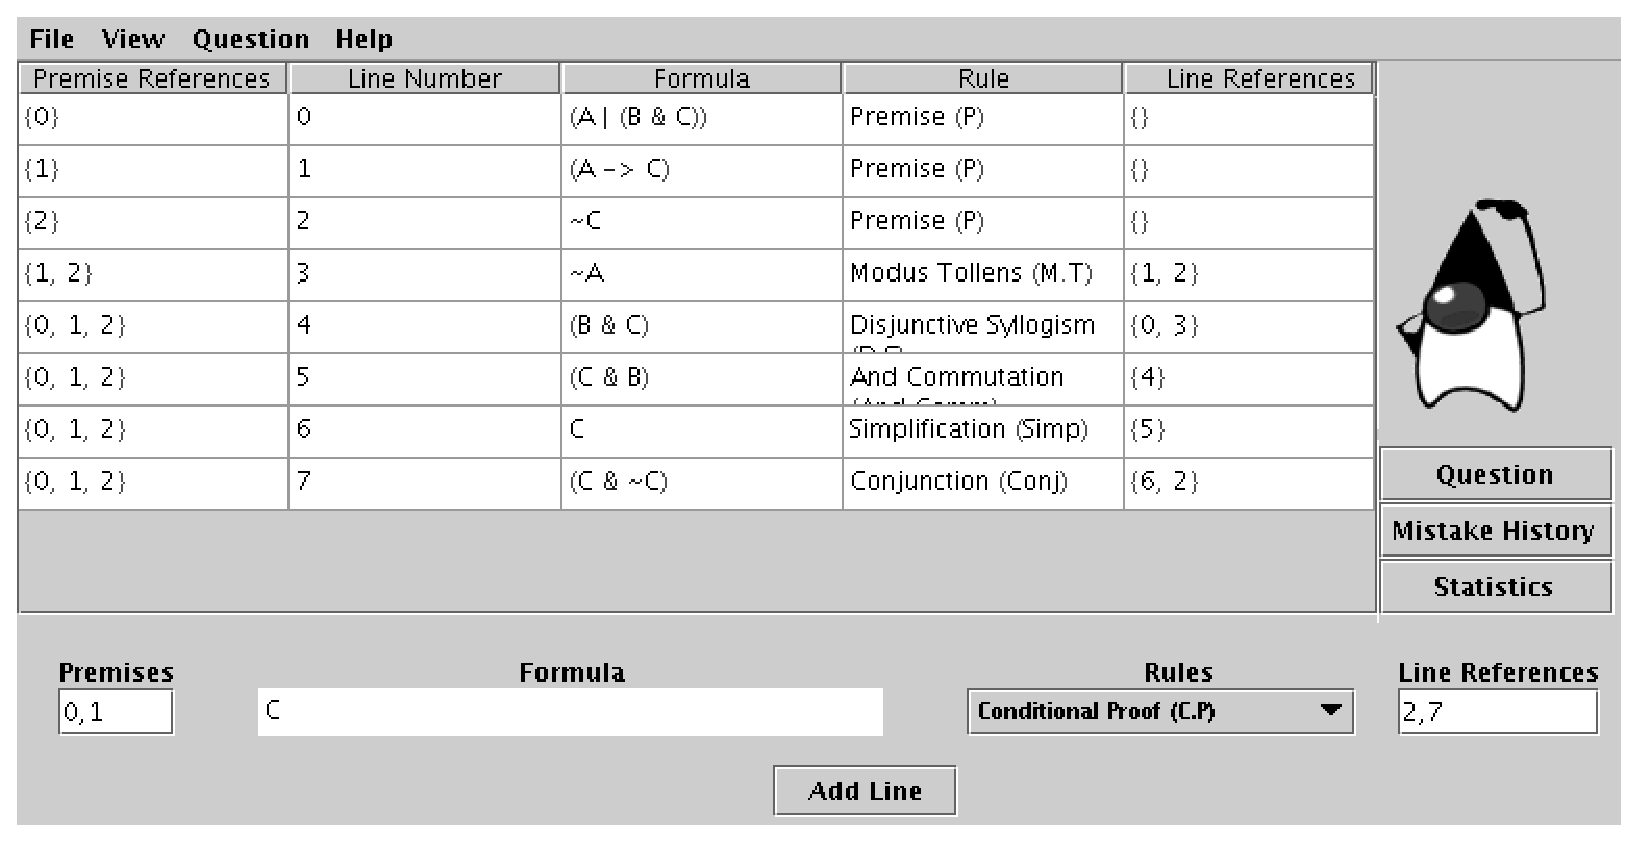
\includegraphics[width=9cm]{screenshot.eps}}
%%%\special{psfile=screenshot.ps hoffset=-15 voffset=-10}% hscale=60 vscale=60}
\caption{Screenshot during an exercise.}
\label{screen}
\end{figure}

For example in Figure \ref{screen}, the student is currently deriving the formula $C$, using the rule {\em Indirect Proof} and the formulae of lines 2 and 7. Because lines 2 and 7 rely respectively on premises {2} and {0,1,2} (as can be seen in the first column of the screen) and {\em Indirect proof} removes the premise 2, the line entered therefore relies on premises {0,1}. It is actually the last step of this exercise, deriving the conclusion. 

At each step, the system checks the validity of the data entered by the student. There are different types of mistakes, and, each of them is labelled with a meaningful title for the teacher. For example, the mistake message {\em Wrong reference lines} means that the student has not provided the right lines of reference the rule applies to. 
  

\subsection{Retrieving implicit information provided by face to face teaching}

%In a context of distance education, teachers do not have anymore the visual information that face to face teaching provides. An obvious example concerns course material. In face to face teaching, they know the course material students are supposed to have seen because it is what they have taught in their lectures. In our information model, storing trails of students through course material allows to retrieve this information.

In face to face teaching, teachers would be aware of students who succeed completing exercises and students who fail, on how students use the tool, in a thoughtful manner or just trying any possible exercise, any possible rule one after the other -- at least as far as classes are not too big.
Experiments with the Logic-ITA  indicate that this kind of information on students' behaviours can be conveyed to teachers.


The aim of the tool is to help students grasp formal proofs. In the
case students  make mistakes but finish successfully exercises,
teachers do not need to worry. Teachers need to be aware of students
not completing successfully exercises since they may have
difficulties. In order to characterize these latter students, a
 k-means clustering \cite{han} has been applied, taking
into account the recorded mistakes. The clustering  yields three
classes. Class 1 is composed of students making few mistakes, class 2
of students making an intermediate number of mistakes and class 3
students making many mistakes, see \cite{akwww04} for more details.
Then several graphs have been produced. A first graph plots {\em
logins} (i.e. student identification) against {\em exercise-id}
(exercise identification).  Thus this graph visualizes the various
exercises attempted by each student. The trend given by this graph is
that students of class 1  attempt more exercises than  students from
class 2 or 3. A second graph plots {\em logins} against {\em
mistake-messages}. The trend given by this graph is that students from
class 2 or 3 make more different kinds of mistakes that students from
class 1. Students from class 1 make the mistakes that are most usually
made by everybody using the tool.  Plotting {\em logins} against {\em
logical-rules} used in the non-completed exercises gave the graph
given in Figure \ref{loginRules}. This graph shows vertical lines for
several students from  class 2 or 3 only, not from class 1. Students
from class 1 constitute the narrow green strip in the middle of the
graph. A vertical line means that all rules have been tried while
doing the exercises.  They suggest that these students have just tried
one rule after the other from the pop-up menu, apparently adopting a
behaviour of "guess and test" strategy. Awareness of these behaviours
may lead teachers to differentiate their pedagogy. 

\begin{figure}[htbp]
{\includegraphics[width=9cm]{login_rule2.eps}}
%% \special{psfile=LoginRule2.ps hoffset=-15 voffset=-10}% hscale=60 vscale=60}
\caption{Plot of Students against Logic Rules.}
\label{loginRules}
\end{figure}


\subsection{Extracting hidden information}

Using Data Mining techniques on students'answers stored in the database can lead to discover  patterns that quite often remain hidden or not well defined otherwise. We have used the association rule algorithm to all the answers from the Logic-ITA to be aware of mistakes often made together while solving exercises. Figure \ref{diagnosis} shows parts of the result, \cite{AK-AIeD} gives more details. 

As an example, the association
{\em Rule can be applied, but deduction incorrect} $\rightarrow $
{\em Premise set incorrect} means that while solving an exercise, if a student makes the mistake {\em Rule can be applied, but deduction incorrect} then s/he makes also the mistake {\em Premise set incorrect}, this association has a support of 60\%. and a confidence of 82\%.
Support makes sure that only mistakes occurring
often enough in the data will be taken into account. Confidence is a measure of how much  $Y$  is really
implied by $X$ in the rule  $X$ $\rightarrow $ $Y$.  


First, we  explain what these mistake messages mean, refering to the example
shown in Figure \ref{screen}. Consider
line 3. If the student  gives
the formula $A$ instead of $~A$, the mistake 
{\em Rule can be applied, but deduction incorrect}
is made.
Indeed, {\em Disjunctive Syllogism} can be applied, but the negated left side of the formula given line 1 can be deduced, as shown in Figure \ref{screen}, not the positive form as written here.  Suppose now that the student gives only 1
in the $Prem.$ field. Then the mistake {\em Premise set incorrect}
is made.
Finally, suppose that the student  gives only 1 in the $Re\!f\!s.$
field. Then a 
{\em Wrong number of line references given} mistake is
 made, because 2 lines of reference are needed.

  
\begin{figure}
\begin{tabular}{|l|c|c|}
\hline
association & supp. & conf.\\
\hline
{\em Rule can be applied, but deduction incorrect} & \ & \ \\
 $\rightarrow $
{\em Premise set incorrect} & 61\% & 82\%\\
\ & \  & \  \\
{\em Premise set incorrect}  & \ & \ \\ 
$\rightarrow $ 
{\em Wrong number of line references given} & 67\% & 87\%\\
\ & \  & \  \\
{\em Rule can be applied, but deduction incorrect}  & \ & \ \\
$\rightarrow $  {\em Wrong number of line references given} & 65\% & 87\%\\
%{\em Premise set incorrect} $\rightarrow $
%{\em Wrong number of line references given}, & \  & \ \\
%{\em Rule can be applied, but deduction incorrect} & 0.56 & 0.73\\
%{\em Rule can be applied, but deduction incorrect},
%{\em Premise set incorrect}& \  & \ \\
%$\rightarrow $
%{\em Wrong number of line references given}& 0.56 &  0.92\\
\hline
\end{tabular}
\caption{Associations found focusing on mistake messages.}
\label{diagnosis}
\end{figure}

The associations found  show relations between
mistakes involving line numbers in the premises
({\em Premise set incorrect}), 
  line numbers in the reference lines a logic rule 
applies to ({\em Wrong number of line references given})
and  incorrect use
 of logic rules ({\em Rule can be applied, but deduction incorrect}).
This confirms what human tutors had sensed.
First, students often have difficulties at grasping
all details required in a proof: one has to provide
not only a logic rule, but also the lines it applies to,
and these are different from the premises involved.
Second, students do not realize at once that there
are two kinds of logic rules:  rules of equivalence that
are applied to one formula only, and  rules of inference
that are mostly applied to two formulas.
Most importantly, rules of
equivalence can be applied to subparts of a formula whereas rules of
inference can only be applied to whole formulae. For example in the
formula $((A \wedge  B) -> C)$ we can validly replace $(A \wedge B)$
 with $(B \wedge A)$ in the formula 
using the rule of equivalence {\em And Commutation} but it is not valid
to deduce $B$ from  $((A \rightarrow B) \rightarrow C)$ and $A$
 using the
rule of inference {\em Modus Ponens}.
Following these findings, presentation of the course material has been revised to put more emphasis on the differences between rules of equivalence
and rules of inference.  

